\documentclass[a4paper,10pt]{ctexart} 

% First, we usually want to set the margins of our document. For this we use the package geometry.
\usepackage[top = 2.5cm, bottom = 2.5cm, left = 2.5cm, right = 2.5cm]{geometry} 
\usepackage[T1]{fontenc}
\usepackage[utf8]{inputenc}

% The following two packages - multirow and booktabs - are needed to create nice looking tables.
\usepackage{multirow} % Multirow is for tables with multiple rows within one cell.
\usepackage{booktabs} % For even nicer tables.

% As we usually want to include some plots (.pdf files) we need a package for that.
\usepackage{graphicx} 

% The default setting of LaTeX is to indent new paragraphs. This is useful for articles. But not really nice for homework problem sets. The following command sets the indent to 0.
% \usepackage{setspace}
% \setlength{\parindent}{0in}
\usepackage{indentfirst}

% Package to place figures where you want them.
\usepackage{float}

% The fancyhdr package let's us create nice headers.
\usepackage{fancyhdr}

\usepackage{amsmath,amsthm,tikz}
\usepackage[hidelinks]{hyperref}
\usetikzlibrary{positioning,patterns}
\usepackage{listings}
\usepackage{color}
\definecolor{dkgreen}{rgb}{0,0.6,0}
\definecolor{gray}{rgb}{0.5,0.5,0.5}
\definecolor{mauve}{rgb}{0.58,0,0.82}
\definecolor{amber}{rgb}{1.0, 0.49, 0.0}
\definecolor{applegreen}{rgb}{0.55, 0.71, 0.0}
\lstset{language=SQL,
  basicstyle={\small\ttfamily},
  belowskip=3mm,
  breakatwhitespace=true,
  breaklines=true,
  classoffset=0,
  columns=flexible,
  commentstyle=\color{dkgreen},
  framexleftmargin=0.25em,
  frameshape={}{yy}{}{}, %To remove to vertical lines on left, set `frameshape={}{}{}{}`
  keywordstyle=\color{amber},
  numbers=none, %If you want line numbers, set `numbers=left`
  numberstyle=\tiny\color{gray},
  showstringspaces=false,
  stringstyle=\color{applegreen},
  tabsize=3,
  xleftmargin =1em
}

% To make our document nice we want a header and number the pages in the footer.

\pagestyle{fancy} % With this command we can customize the header style.

\fancyhf{} % This makes sure we do not have other information in our header or footer.

\lhead{\footnotesize 数据库原理(H) Project 2 报告}% \lhead puts text in the top left corner. \footnotesize sets our font to a smaller size.

%\rhead works just like \lhead (you can also use \chead)
\rhead{\footnotesize 吴梦轩} %<---- Fill in your lastnames.

% Similar commands work for the footer (\lfoot, \cfoot and \rfoot).
% We want to put our page number in the center.
\cfoot{\footnotesize \thepage} 

\begin{document}

\begin{center}
	{\Large \bf 数据库原理(H) Project 2 报告}
	\vspace{2mm}

	{\bf 吴梦轩}
    \vspace{2mm}

	{\bf 12212006}
		
\end{center}  

\vspace{0.4cm}

\section{数据库设计}

\subsection{实体关系图}

我使用的是 crow's foot 符号,并将实体表的表头用单独的颜色标出,关系表的表头统一用紫色标出。

\begin{figure}[H]
    \centering
    \includegraphics[width=0.8\textwidth]{Database ER diagram (crow's foot).png}
    \caption{实体关系图}
\end{figure}

\newpage
\subsection{数据库可视化}

由于设计的数据库不使用外键,所以在可视化时,我将实体表和关系表分开显示。

\begin{figure}[H]
    \centering
    \includegraphics[width=0.8\textwidth]{Visualization.png}
    \caption{数据库可视化}
\end{figure}

\subsection{数据库设计简述}

本次设计中,我查阅并尽可能遵守了阿里巴巴 Java 开发手册\footnote{Java 手册界面 - 阿里云开发者社区,\url{https://developer.aliyun.com/special/tech-java}}中的规范,具体见下文。

本数据库共有3个实体表和6个关系表,其中实体表为 \texttt{user}、\texttt{video}、\texttt{danmu},
关系表为 \texttt{user\_like\_danmu}、\texttt{user\_watch\_video}、\texttt{user\_coin\_video}、\texttt{user\_like\_video}、\texttt{user\_collect\_video}和\texttt{user\_follow},通过表名表示了实体之间的关系。
此设计遵守阿里巴巴 Java 开发手册中的规范有:
\begin{itemize}
    \item 表名、字段名必须使用小写字母或数字,禁止出现数字开头
    \item 表名不使用复数名词
\end{itemize}

考虑到本数据库是为大型公司而设计,需要存储大量的数据且有数据审计的需求,我采用了无外键,软删除的设计。
其具体做法为:在每个实体表和关系表中都加入了一个 \texttt{is\_deleted} 字段,默认为\texttt{false},用于标记该条记录是否被删除。
在删除实体时,手动更新该实体及其相关的关系表中的所有记录的 \texttt{is\_deleted} 字段为 \texttt{true}。
为保证查询效率,我使用了部分索引,即只对 \texttt{is\_deleted} 字段为 \texttt{false} 的记录建立索引。
此设计遵守阿里巴巴 Java 开发手册中的规范有:
\begin{itemize}
    \item 表达是与否概念的字段,必须使用 \texttt{is\_xxx} 的方式命名
    \item 不得使用外键与级联
\end{itemize}

在数据库权限管理方面,由于我将每个功能都封装成了一个数据库\texttt{function},所以只需要对于不同的\texttt{role}赋予对应的\texttt{function}的\texttt{execute}权限即可。
具体而言,可以考虑以下几种\texttt{role}:
\begin{itemize}
    \item 访客:查询弹幕\texttt{displayDanmu}、获得推荐视频\texttt{generalRecommendation}和注册\texttt{register}权限
    \item 普通用户:在访客的基础上,获得投稿视频\texttt{postVideo}、更改视频信息\texttt{updateVideoInfo}、投币\texttt{coinVideo}、点赞\texttt{likeVideo}、收藏\texttt{collectVideo}、关注\texttt{follow}、发送弹幕\texttt{sendDanmu}、点赞弹幕\texttt{likeDanmu}、获得个性化推荐视频\texttt{recommendVideoForUser}、获得朋友推荐\texttt{recommendFriend}、删除视频\texttt{deleteVideo}和删除账号\texttt{deleteAccount}权限(此处只能删除自己的视频和账号)
    \item 超级用户:在普通用户的基础上,获得审核视频\texttt{reviewVideo}权限,且此时可以删除任意视频和任意普通用户的账号
    \item 数据库管理员/数据分析师:在超级用户的基础上,获得检查用户是否合法\texttt{validateUserInfo}、查看视频热点\texttt{getHotSpot}和查看视频观看率\texttt{getAverageViewRate}权限,同时拥有所有表的select权限
\end{itemize}

本数据库遵守了第三范式,即每个非主键属性都不传递依赖于主键,每个非主键属性都直接依赖于主键。

\section{数据库特殊实现}

我的报告主要包含以下几个部分,其主要部分为探索软删除的实现方式以及两种实现方式的优缺点。
结构如下:
\begin{itemize}
    \item 软删除的设计
        \begin{itemize}
            \item 历史表方法
                \begin{itemize}
                    \item Bloat膨胀问题
                    \item Bloat膨胀的原因:对PostgreSQL的MVCC机制的探索
                \end{itemize}
            \item 标记删除方法
                \begin{itemize}
                    \item 通过部分索引保证查询效率
                    \item 额外探索:Postgres Query Planner如何使用索引
                \end{itemize}
        \end{itemize}
    \item 数据库性能优化
    \item 数据库安全性优化
    \item 其他优化与设计
\end{itemize}

\subsection{软删除}

软删除 (Soft Delete)是相对于硬删除 (Hard Delete)来说的,又称逻辑删除,指的是在数据库中,不是真正地删除数据,而是通过某种标记使得数据被过滤掉,从而达到删除的效果。
软删除的存在很多时候不仅是为了数据审计或数据恢复,而是因为真实世界中往往不存在真正的删除,而是数据发生了存在状态的改变,并且在新的状态下可能产生了新的价值。
Udi Dahan 曾发表文章\textit{Don't Delete - Just Don't} \footnote{Udi Dahan, \textit{Don't Delete - Just Don't}, \url{https://udidahan.com/2009/09/01/dont-delete-just-dont/}}来阐述这一观点。
\begin{itemize}
    \item 订单不是被“删除”的,而是被取消的,并且可能由于过晚取消而产生了违约金
    \item 员工不是被“删除”的,而是被解雇的,并且公司可能需要为其支付一定的补偿金
    \item (需要招聘的)职位不是被“删除”的,而是被填补了或者不再需要了
\end{itemize}

\vspace{0.7cm}
并且,即使被删除的数据不会产生新的价值,也并不能简单的级联删除:
\begin{itemize}
    \item 问题:如果一个商品被下架了,我们能够直接级联删除它吗?
    \begin{itemize}
        \item 答:不能。如果我们直接级联删除了该商品,那么所有购买了该商品的订单、仓库中该商品的库存记录以及该商品的进货记录都会被删除,这显然是不合理的。
    \end{itemize}
\end{itemize}

Udi Dahan 最后总结道:\textbf{The real world doesn't cascade!} 
我们需要更合理的方式来处理数据的删除,也就是软删除。

我对软删除的实现方式进行了探索,主要有两种方法:
\begin{enumerate}
    \item 为每个表建立一个新的历史表,用于存储被删除的记录,使用\texttt{trigger}将删除的记录插入到历史表中
    \item 在每个表中加入一个新字段,用于标记该条记录是否被删除
\end{enumerate}

接下来我将对这两种方法进行详细的说明。

\subsubsection{方法一:历史表}

采用历史表的方式是最为简单的,我在最初的设计中也想过采用这种方式。
其优点是:
\begin{itemize}
    \item 逻辑清晰,易于理解
    \item 软删除的记录和原记录分开存储,不会影响查询未删除记录的效率
    \item 不需要对SQL语句进行修改,每次删除时\texttt{trigger}自动将记录插入到历史表中
\end{itemize}

\vspace{0.7cm}
看上去这种方式是完美的,但是我在lab课学习了如何查看表和索引的大小后,意外发现了一个问题,并最终让我放弃了这种方式。

\begin{center}
    \textbf{为什么删除记录后表的大小没有变化?}
\end{center}

对此我进行了一些实验:创建一个\texttt{exp}表,包含两个字段:主键\texttt{id}和\texttt{name},并插入了一百万条记录。

\begin{lstlisting}[language=SQL]
    CREATE TABLE exp
    (
        id   INT PRIMARY KEY,
        name VARCHAR(20)
    );
    
    INSERT INTO exp
    SELECT i, (floor(random() * 1000))::text
    FROM generate_series(1, 1000000) as i;
\end{lstlisting}

然后我删除了id为偶数的记录,并记录了删除前后表与索引的大小。

\begin{lstlisting}[language=SQL]
    DELETE
    FROM exp
    WHERE id % 2 = 0;
    
    SELECT pg_size_pretty(pg_relation_size('exp')) AS table_size, pg_size_pretty(pg_indexes_size('exp')) AS index_size;
\end{lstlisting}

结果发现,删除前后表和索引的大小完全没有变化!
\begin{center}
    \begin{tabular}{ccc}
        \toprule
        \textbf{操作} & \textbf{表大小} & \textbf{索引大小} \\
        \midrule
        删除前 & 35 MB & 21 MB \\
        删除后 & 35 MB & 21 MB \\
        \bottomrule
    \end{tabular}
\end{center}

经过搜索,我发现了原因:\textbf{PostgreSQL不会立即回收删除的空间},已删除的记录仍然被保留在表中,直到\texttt{VACUUM}命令运行时才会被回收,这导致表的大小不会立刻减少。
这种现象被称为\textbf{Bloat},即膨胀。
这是为了MVCC (Multi-Version Concurrency Control,多版本并发控制)的实现而做出的妥协。

\vspace{0.7cm}
为了更好的说明这一现象,我将首先介绍MVCC的实现原理:

当很多人同时操作数据库时,可能同时存在读写操作。
如果同一条记录在被读取时被修改了,那么读取到的数据可能是不完整的,或者是不一致的。
\begin{figure}[H]
    \centering
    \resizebox{\linewidth}{!}{
        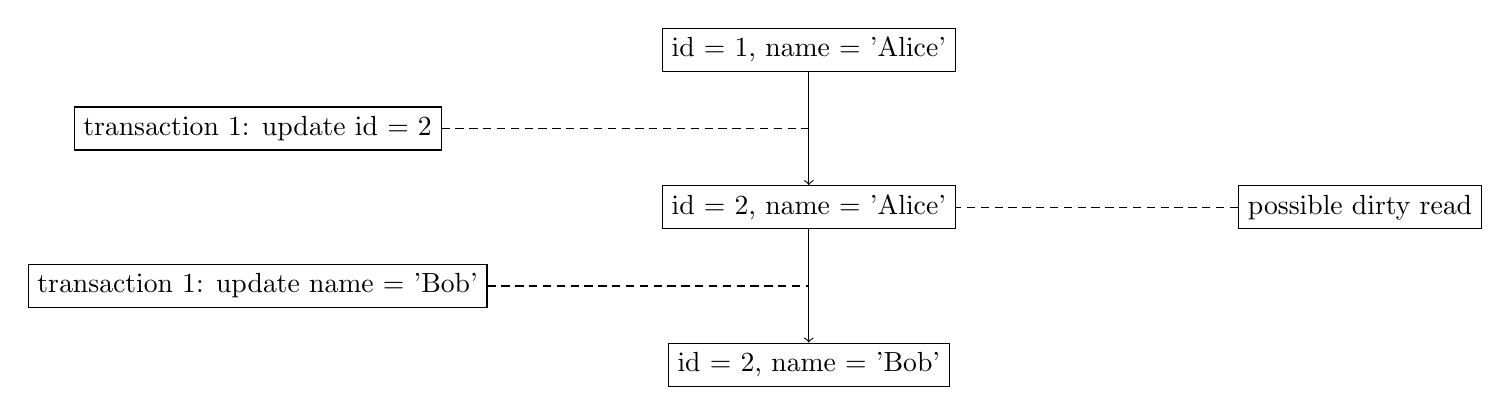
\begin{tikzpicture}
            \draw (0,0) node [draw, rectangle] (A) {id = 1, name = 'Alice'};
            \draw (-7,-1) node [draw, rectangle] (t1 1) {transaction 1: update id = 2};
            \draw (0,-2) node [draw, rectangle] (B) {id = 2, name = 'Alice'};
            \draw (-7,-3) node [draw, rectangle] (t1 2) {transaction 1: update name = 'Bob'};
            \draw (0,-4) node [draw, rectangle] (C) {id = 2, name = 'Bob'};
            \draw (7,-2) node [draw, rectangle] (t2 1) {possible dirty read};

            \draw[->] (A) -- (B);
            \draw[->] (B) -- (C);
            \draw[densely dashed] (t1 1) -- (0,-1);
            \draw[densely dashed] (t1 2) -- (0,-3);
            \draw[densely dashed] (t2 1) -- (B);
        \end{tikzpicture}
    }
    \caption{不约束并发读写可能导致的问题}
\end{figure}

为了避免这种情况的发生,数据库需要对读写操作进行并发控制。
最简单的解决方式是将正在被修改的记录锁定,不允许读取,直到修改完成后才解除锁定,但是这种方式会导致并发性能极差。
因此,PostgreSQL 采用了 MVCC 的方式来实现并发控制:
\begin{itemize}
    \item 每个\texttt{transaction}都有一个唯一的\texttt{transaction id} (又称\texttt{xid}),用于唯一标记该\texttt{transaction}
    \item 当\texttt{transaction}对某一行记录进行修改时,将为该行记录创建一个新版本。只对新版本进行修改,旧版本将被保留但标记为已删除
    \item 在底层,每个版本由一个tuple对应存储。每个tuple的header中都有两个字段:\texttt{xmin}和\texttt{xmax},分别表示创建该tuple的\texttt{xid}和删除该tuple的\texttt{xid},未被删除的记录的\texttt{xmax}为\texttt{0}。
    \item 每个\texttt{transaction}通过读取tuple的header,可以判断该tuple是否在该\texttt{transaction}中可见
\end{itemize}

这样,由于任何修改操作都不会直接修改原有的记录,所以读取操作不会被阻塞,从而实现了并发控制。
我将通过\texttt{pageinspect}扩展来查看tuple的各项属性,并配合实验阐释MVCC的实现原理。

先创建一个\texttt{transaction\_test}表,并插入一条数据{id = 1, name = 'a'}。
\begin{lstlisting}[language=SQL]
    CREATE TABLE transaction_test
    (
        id   INT PRIMARY KEY,
        name VARCHAR(20)
    );

    INSERT INTO transaction_test
    VALUES (1, 'a');
\end{lstlisting}

使用\texttt{pageinspect}扩展查看该表
\begin{center}
    \begin{lstlisting}[language=SQL]
        SELECT lp, t_xmin, t_xmax, t_ctid, t_infomask
        FROM heap_page_items(get_raw_page('transaction_test', 0));
    \end{lstlisting}
\end{center}

可得:
\begin{center}
    \begin{tabular}{ccccccc}
        \toprule
        lp & t\_xmin & t\_xmax & t\_ctid & t\_infomask & id & name \\
        \midrule
        1 & 71986 & 0 & (0,1) & 2050 & 1 & a \\
        \bottomrule
    \end{tabular}
\end{center}
\textit{我手动加入了tuple对应的内容,方便理解}

表格解读:
\begin{itemize}
    \item \texttt{lp}为该tuple在当前page中的编号,目前为第一个tuple。
    \item \texttt{t\_ctid}指向了当前tuple最新的版本的位置,当前指向第0个page的第1个tuple,即指向了自己。
    \item \texttt{t\_infomask}的解读较为复杂,该字段可以解读出\texttt{t\_xmin}与\texttt{t\_xmin}各自对应的\texttt{transaction}是否已经提交或被放弃(rollback),具体为:将其转化为二进制后,若第9位为1,则\texttt{t\_xmin}对应的\texttt{transaction}已经提交,若第10位为1,则\texttt{t\_xmin}对应的\texttt{transaction}被放弃,若第11位为1,则\texttt{t\_xmax}对应的\texttt{transaction}已经提交,若第12位为1,则\texttt{t\_xmax}对应的\texttt{transaction}被放弃。
          目前值为2050,可知\texttt{t\_xmax}对应的\texttt{transaction}被放弃,即该记录未被删除。
\end{itemize}
\textit{接下来,我将在\texttt{t\_xmin}和\texttt{t\_xmax}旁用a表示该\texttt{transaction}被放弃,用c表示该\texttt{transaction}已经提交,用r表示该\texttt{transaction}正在运行。}

然后我开启两个\texttt{transaction},并使用\texttt{txid\_current()}函数查看当前\texttt{transaction}的\texttt{xid}。
得知\texttt{transaction 1}的\texttt{xid}为\texttt{71989},\texttt{transaction 2}的\texttt{xid}为\texttt{71990}。
在\texttt{transaction 1}中,我将id为1的记录的name修改为'b',此时再次查看该表,可得:
\begin{center}
    \begin{tabular}{ccccccc}
        \toprule
        lp & t\_xmin & t\_xmax & t\_ctid & t\_infomask & id & name \\
        \midrule
        1 & 71986(c) & 71989(r) & (0,2) & 258 & 1 & a \\
        2 & 71989(r) & 0(a) & (0,2) & 10242 & 1 & b \\
        \bottomrule
    \end{tabular}
\end{center}

可以看到,因为\texttt{transaction 1}修改了id为1的记录,所以该记录被复制了一份,放入到了第2个tuple中。
原本的记录已经过时,应该被标记为删除,所以其\texttt{xmax}被设置为\texttt{71989},表示该记录被\texttt{transaction 1}删除。
同时,第1个tuple的\texttt{t\_ctid}被修改为(0,2),指向了第2个tuple,表示第1个tuple代表的该行记录的最新版本为第2个tuple。

在\texttt{transaction 2}查看该表时,从编号为1的tuple的\texttt{t\_infomask}中得知,该记录虽然已经被标记为删除(\texttt{xmax}不为0),但是其\texttt{xmax}对应的\texttt{transaction}还在运行,所以该记录仍然可见。
从编号为2的tuple的\texttt{t\_infomask}中得知,该tuple的\texttt{xmin}对应的\texttt{transaction}还在运行,即该记录还未提交,所以对\texttt{transaction 2}来说,这条记录不可见。
此时就实现了MVCC的并发控制:\texttt{transaction 1}修改后,只能看到tuple 2,但此时\texttt{transaction 2}仍然可以看到tuple 1,看不到tuple 2。

在\texttt{transaction 1}提交后,再次查看该表,可得:
\begin{center}
    \begin{tabular}{ccccccc}
        \toprule
        lp & t\_xmin & t\_xmax & t\_ctid & t\_infomask & id & name \\
        \midrule
        1 & 71986(c) & 71989(c) & (0,2) & 1282 & 1 & a \\
        2 & 71989(c) & 0(a) & (0,2) & 10498 & 1 & b \\
        \bottomrule
    \end{tabular}
\end{center}

此时各个tuple的\texttt{t\_infomask}被更新,使得编号为1的tuple不再可见,编号为2的tuple可见。
此时编号为1的tuple已永远不会被访问,成为了dead tuple。

删除记录的方式与修改记录的方式类似,只是不会创建新的tuple,而是直接将\texttt{xmax}设置为当前\texttt{transaction}的\texttt{xid},并将\texttt{t\_infomask}设置为1282,表示该记录已经被删除。
例如以下代码:
\begin{lstlisting}[language=SQL]
    CREATE TABLE transaction_test
    (
        id   INT PRIMARY KEY,
        name VARCHAR(20)
    );

    INSERT INTO transaction_test
    VALUES (1, 'a');

    DELETE
    FROM transaction_test
    WHERE id = 1;

    SELECT lp, t_xmin, t_xmax, t_ctid, t_infomask
    FROM heap_page_items(get_raw_page('transaction_test', 0));
\end{lstlisting}

其运行结果为:
\begin{center}
    \begin{tabular}{ccccccc}
        \toprule
        lp & t\_xmin & t\_xmax & t\_ctid & t\_infomask & id & name \\
        \midrule
        1 & 72004(c) & 72004(c) & (0,1) & 1282 & 1 & a \\
        \bottomrule
    \end{tabular}
\end{center}

可见,由于在删除和修改记录时,都会创建新的版本,所以表的大小会不断增加。
对应的,表上的索引因为也需要支持MVCC,被删除的记录也会被加入到索引中,其大小也会不断增加。

\vspace{0.7cm}

说了这么多MVCC的实现原理,现在回到我们的问题:为什么不选择历史表的方式来实现软删除?
因为\textbf{Bloat膨胀}问题在还设计有历史表的情况下只会更加严重,被删除的tuple不仅会占用原表的空间,还会占用历史表的空间。
更重要的是,索引中也会存在大量的被删除的记录,导致索引的大小不断增加的同时,查询效率也会不断降低。
曾有过通过\texttt{VACUUM}命令删除了超过70GB的dead tuple和20GB的无效索引的例子\footnote{Haki Benita, The Unexpected Find That Freed 20GB of Unused Index Space, \url{https://hakibenita.com/postgresql-unused-index-size}},
如果在该设计中还加入了历史表,那么就会导致额外的90GB的空间被占用。

\vspace{0.7cm}
如果仅仅是占用空间过大的问题,那么\texttt{VACUUM}命令不可以解决吗?
我认为,\texttt{VACUUM}操作同样存在一些问题使其不符合视频公司的需求:
\begin{itemize}
    \item \texttt{VACUUM}命令会删除dead tuple,但是由于删除的位置是随机的,有效信息将会被分散到磁盘上的各个地方,导致磁盘碎片化,进而影响查询效率
    \item \texttt{VACUUM FULL}命令会真正释放磁盘空间并重新排列数据,但极为耗时且会阻塞读写操作,并不适合视频公司这种需要实时更新的场景
\end{itemize}

综上,我放弃了通过创建历史表的方式来实现软删除的想法。

\subsubsection{方法二:标记删除}

在放弃了历史表的方式后,我开始探索另一种方式:在每个表中加入一个新字段,用于标记该条记录是否被删除。
通过以下方法可以快速将一般的数据库设计改为软删除的设计:
\begin{itemize}
    \item 在每个表中加入一个新字段\texttt{is\_deleted},用于标记该条记录是否被删除
    \item 为每一个表创建一个\texttt{view},只显示\texttt{is\_deleted}为\texttt{false}的记录,并将原来的sql语句中的表名替换为\texttt{view}名(如果服务已经发布,则应反向操作,将\texttt{view}的名字改为原来的表名)
    \item 在执行删除操作时,手动级联更新所有相关的表中的\texttt{is\_deleted}字段(此处需要将原来的delete语句改为update语句)
\end{itemize}
在实践中,标记字段也存在一些变种。如将标记字段改为\texttt{timestamp}类型,用于记录删除的时间,或者将标记字段改为\texttt{smallint}类型,可以存储不同的删除状态或者不同等级的可见性。

\vspace{0.7cm}
前面所提到的改动都相对简单。在这种设计中,所遇到的最大挑战来自于主键和索引的设计:如何设计主键和索引,使得查询效率最高?

\textbf{问题一:唯一性约束如何实现?}

主键和其他unique约束的唯一性应该只对未被删除的记录进行约束,此时原有的设计已经不满足要求。
假设我们设计了一个不允许重复姓名存在的用户表,并只是简单的在表中增加了\texttt{is\_deleted}字段。
很明显,这样的设计是不合理的:
姓名为Alice的用户被删除后,仍然不能再创建一个姓名为Alice的用户。

一开始我想到的解决方案是:将\texttt{is\_deleted}字段也加入到unique约束中,即:
\begin{center}
    \begin{lstlisting}[language=SQL]
        CREATE TABLE exp
        (
            id          INT,
            name        VARCHAR(20),
            is_deleted BOOLEAN DEFAULT FALSE,
            PRIMARY KEY (id),
            UNIQUE (name, is_deleted)
        );
    \end{lstlisting}
\end{center}

但是这样的设计也存在问题:
\begin{itemize}
    \item 如果已经有一个姓名为Alice的用户被删除了,此时可以创建一个姓名为Alice的用户,但是却不能删除这个新创建的用户。
    \item \textbf{unique约束对应的索引包含了所有的记录,包括已经被删除的记录(完全相同的Bloat膨胀问题)}
\end{itemize}

\vspace{0.7cm}
\textbf{问题二:查询效率如何保证?}

在只需要检索一条记录时,原有的主键索引似乎完全可以满足要求。
借用上面的例子,如果我们需要查询id为1的用户的姓名,使用\texttt{EXPLAIN}给出的执行计划如下表示,PostgreSQL会先使用主键索引找到id为1的记录,然后再检查该记录的\texttt{is\_deleted}字段是否为\texttt{false},最后返回\texttt{name}字段。

但是,如果检索结果有多条记录,那么查询效率就会大大降低:
比如在本次设计中,有一个\texttt{get\_user\_info}的方法,需要返回某个用户观看的所有视频的bv号。
如果我们不改动原有设计,即将\texttt{user\_watch\_video}表中的用户编号\texttt{mid}和视频编号\texttt{bv}作为复合主键,
那么在查询某个用户观看的所有视频时,PostgreSQL需要通过主键先找到该用户的所有观看记录,再对每条记录进行一次检查,判断该记录是否被删除,最后返回所有未被删除的记录。
\begin{center}
    \begin{lstlisting}[language=SQL]
        EXPLAIN
        SELECT bv
        FROM user_watch_video
        WHERE mid = 1 AND is_deleted = FALSE;

        QUERY PLAN
        Bitmap Heap Scan on user_watch_video  (cost=4.60..92.76 rows=23 width=13)
            Recheck Cond: (mid = 1)
            Filter: (NOT is_deleted)
            ->  Bitmap Index Scan on user_watch_video_pk  (cost=0.00..4.60 rows=23 width=0)
                Index Cond: (mid = 1)
    \end{lstlisting}
\end{center}

很明显,在已经删除的记录较多的情况下,这样的查询效率是很低的。
更重要的是,\textbf{这么做的效率一定低于原先硬删除的设计},因为硬删除的设计中,表中的记录都是未被删除的,不需要进行额外的检查。

\vspace{0.7cm}
经过搜索,我发现了一个解决方案:\textbf{部分索引(Partial Index)}。

部分索引是指只对满足某一条件的记录建立索引,不满足条件的记录不会被加入到索引中。
如果对\texttt{is\_deleted}为\texttt{false}的数据建立部分索引,则可以完全排除掉已经被删除的记录,既减小了索引的大小,又可以实现只对未被删除的记录建立unique约束。
例如在本次设计中,\texttt{user\_watch\_video}表中的索引即为部分索引:
\begin{center}
    \begin{lstlisting}[language=SQL]
        CREATE INDEX idx_user_watch_video_mid_bv
        ON user_watch_video (mid, bv)
        WHERE is_deleted = FALSE;
    \end{lstlisting}
\end{center}

如果此时再次查询某个用户观看的所有视频,PostgreSQL会直接使用部分索引,而不是先使用主键索引再进行检查:
\begin{center}
    \begin{lstlisting}[language=SQL]
        EXPLAIN
        SELECT bv
        FROM user_watch_video
        WHERE mid = 1;

        QUERY PLAN
        Index Only Scan using idx_user_watch_video_mid_bv on user_watch_video  (cost=0.42..4.83 rows=23 width=13)
            Index Cond: (mid = 1)
    \end{lstlisting}
\end{center}

可以从两次查询的执行计划的\texttt{cost}字段看出,使用部分索引的查询效率是原来的二十倍以上,而实际测试时更能达到数百倍!
在设置和不设置部分索引的情况下,分别执行不同次数的\texttt{get\_user\_info}方法,得到的结果如下:
\begin{center}
    \begin{tabular}{lccc}
        \toprule
        \textbf{记录数量} & \textbf{不使用部分索引(单位:毫秒)} & \textbf{使用部分索引(单位:毫秒)} & \textbf{提升效率} \\
        \midrule
        100 & 18465 & 199 & 97倍 \\
        1000 & 198102 & 363 & 545倍 \\
        10000 & 1948565 & 2206 & 883倍 \\
        \bottomrule
    \end{tabular}
\end{center}

此时,我们已经得到了很好的标记删除解决方案。

\vspace{1.5cm}
\textbf{额外探索:索引}

在使用部分索引的前提下,我发现了一些奇怪的现象:
PostgreSQL在使用了部分索引进行\texttt{Bitmap Index Scan}的前提下,仍然执行了recheck操作,而且recheck操作的代价很大。
例如,在一次update操作中,使用\texttt{EXPLAIN ANALYZE}查看执行计划如下:
\begin{center}
    \begin{lstlisting}[language=SQL]
        EXPLAIN ANALYZE
        UPDATE user_watch_video
        SET is_deleted = true
        WHERE mid = 75
          AND is_deleted = false;

        QUERY PLAN
        Update on user_watch_video  (cost=4.60..92.76 rows=0 width=0) (actual time=2.635..2.636 rows=0 loops=1)
        ->  Bitmap Heap Scan on user_watch_video  (cost=4.60..92.76 rows=23 width=7) (actual time=0.046..0.320 rows=26 loops=1)
            Recheck Cond: ((mid = 75) AND (NOT is_deleted))
            Filter: (NOT is_deleted)
            Heap Blocks: exact=26
            ->  Bitmap Index Scan on idx_user_watch_video_mid_bv  (cost=0.00..4.60 rows=23 width=0) (actual time=0.023..0.023 rows=26 loops=1)
                Index Cond: (mid = 75)
    \end{lstlisting}
\end{center}

在这个例子中,我希望删除用户75的所有观看记录(在软删除中转化为update操作)。
可以看到,PostgreSQL首先使用了部分索引\texttt{idx\_user\_watch\_video\_mid\_bv},定位到了用户75的所有未被删除的观看记录。
按理来说,此时索引返回的记录中\texttt{is\_deleted}一定为\texttt{false},但是PostgreSQL仍然在上一级的节点中进行了recheck操作,再次检查\texttt{is\_deleted}字段是否为\texttt{false}。
并且recheck操作的代价很大,占用了绝大部分的执行时间(预计cost中占95\%,实际时间中占85\%)

我产生了两个疑问:
\begin{enumerate}
    \item 为什么有可以直接使用的索引,却不执行\texttt{Index Only Scan},而是执行\texttt{Bitmap Index Scan}和\texttt{Bitmap Heap Scan}?
    \item 在部分索引保证了条件满足的情况下,为什么仍然需要进行recheck操作?
\end{enumerate}

\textbf{问题一:为什么不执行\texttt{Index Only Scan}?}

由于这个问题和读写性能有关,需要回到数据库底层的存储结构上来解释。

\begin{figure}[H]
    \centering
    \includegraphics[width=\linewidth]{pagelayout.png}
    \caption{Page结构图\protect\footnotemark} 
\end{figure}
\footnotetext{PostgreSQL Documentation, \textit{storage-page-layout}, \url{https://www.postgresql.org/docs/current/storage-page-layout.html}}

在PostgreSQL中,每个表都被分为多个固定大小为8KB的Page,每个Page中包含了多个tuple(即图中的item)。
每个tuple被分为header和数据两部分,header中存有一个指针指向数据。
索引中存放的是指向tuple的指针。

此处需要介绍另外一个概念:correlation,即相关性。
索引采用的是B+树的结构,但是在树中相邻的两个节点在磁盘上并不一定相邻。
相关性反应了数据在树上的顺序和在磁盘上的顺序之间的差异,其值在-1到1之间,值越大则顺序越接近,具体值可以从\texttt{pg\_stats}视图中查看。

为何需要引入相关性这一概念呢?因为机械硬盘的顺序读写速度远大于随机读写速度,一般来说可以达到100倍以上(随机读写时机械硬盘需要反复移动磁头)。
使用\texttt{Index Only Scan}时,PostgreSQL会直接按照索引给出的顺序依次读取tuple。
如果相关性很大,则按照索引给出的tuple顺序进行读取几乎就是顺序读取,速度很快。
\begin{figure}[H]
    \centering
    \includegraphics[width=0.8\linewidth]{sequential read.png}
    \caption{顺序读取\protect\footnotemark} 
\end{figure}

\footnotetext{Habr, \textit{Queries in PostgreSQL. Index scan}, \url{https://habr.com/en/companies/postgrespro/articles/666974/}}

但是当相关性很小时,索引给出的tuple顺序和磁盘上的顺序差异很大,此时几乎变为了随机读取:
\begin{figure}[H]
    \centering
    \includegraphics[width=0.8\linewidth]{random read.png}
    \caption{随机读取}
\end{figure}

如果相关性过小,PostgreSQL会放弃使用\texttt{Index Only Scan},而是使用\texttt{Bitmap Index Scan}和\texttt{Bitmap Heap Scan}。
其原理为:首先将所有的tuple指针所在的page读取到内存中,然后生成一个\texttt{Bitmap},其中每个bit代表相应该位置的tuple是否满足条件。
最后,根据\texttt{Bitmap}中的信息,从内存中读取相应的tuple。
这样做的好处是:由于page本身是连续存储的8KB数据,读取单独的page时可以使用顺序读取。
并且生成\texttt{Bitmap}的过程相当于对tuple进行了一次排序,使得读取tuple时的顺序更加接近顺序读取。

\begin{figure}[H]
    \centering
    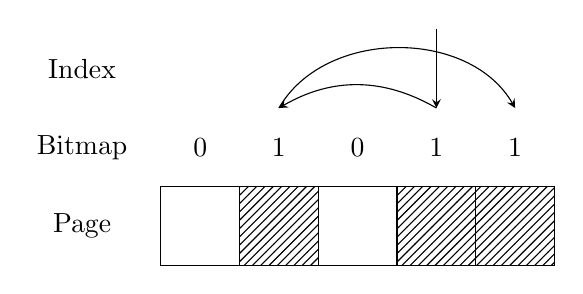
\begin{tikzpicture}
        \draw (0,0) -- (5,0) -- (5,1) -- (0,1) -- cycle;
        \draw (1,0) -- (1,1);
        \draw (2,0) -- (2,1);
        \draw (3,0) -- (3,1);
        \draw (4,0) -- (4,1);
        \draw (0.5,1.5) node {0};
        \draw (1.5,1.5) node {1};
        \draw (2.5,1.5) node {0};
        \draw (3.5,1.5) node {1};
        \draw (4.5,1.5) node {1};
        \draw[pattern={north east lines}] (1,0) -- (2,0) -- (2,1) -- (1,1) -- cycle;
        \draw[pattern={north east lines}] (3,0) -- (4,0) -- (4,1) -- (3,1) -- cycle;
        \draw[pattern={north east lines}] (4,0) -- (5,0) -- (5,1) -- (4,1) -- cycle;
        \draw [-stealth] (3.5,3) -- (3.5,2); 
        \draw [-stealth] (3.5,2) to[out=150,in=30] (1.5,2); 
        \draw [-stealth] (1.5,2) to[out=60,in=120] (4.5,2);
        \draw (-1,0.5) node {Page};
        \draw (-1,1.5) node {Bitmap};
        \draw (-1,2.5) node {Index};
    \end{tikzpicture}
    \caption{Bitmap 示意图}
\end{figure}


附:
PostgreSQL在估算随机读取和顺序读取的代价时,使用的参数\texttt{random\_page\_cost}和\texttt{seq\_page\_cost}分别为4和1。
此数值可以由用户自行修改,例如在随机读写和顺序读写性能差异不大的固态硬盘上,可以将其修改为相同的值。

\vspace{0.7cm}
\textbf{问题二:为什么需要进行recheck操作?}

由问题一可知,进行\texttt{Bitmap Index Scan}需要将目标tuple所在的page读取到内存中。
当page数量过多时,内存开销会很大。
如果PostgreSQL预估使用内存会超过\texttt{work\_mem}的值(默认为4 MB),将转为lossy模式。
在此模式下,原先\texttt{Bitmap}中每个bit对应一个tuple,现在每个bit对应一个page,即改为找出所有包含满足条件的tuple的page。
这样做的好处是:内存开销大大减小,但是获得的page中可能存在一些不满足条件的tuple,需要进行recheck操作。

是否执行lossy模式可以通过\texttt{EXPLAIN ANALYZE}得知,如前文所提到的例子中有一行:\texttt{Heap Blocks: exact=26}。
这表示有26个page是直接对每个tuple生成\texttt{Bitmap}。如果执行了lossy模式,将会显示为:\texttt{exact = ..., lossy = ...}。
即使没有执行lossy模式,仍然会在执行计划中显示recheck操作,但实际运行时不会进行。

\subsection{数据库性能优化}

在此次的项目中,针对不同类型的方法,我采用了不同的优化策略。
但其核心目标可以被总结为:
\begin{itemize}
    \item 减少Java端与数据库连接的次数
    \item 减少Java端与数据库传输的数据量
\end{itemize}

\subsubsection{数据导入}

数据导入部分,我采用的策略有:批处理,多线程插入,多值插入,以及删除与重建索引。

\textbf{批处理与多值插入}

使用批处理功能前,Java端每发送一条SQL语句,都需要等待数据库返回结果,之后才能发送下一条SQL语句。
而在批处理中,Java端可以一次性发送多条SQL语句,并一次性接收多条SQL语句的结果,减少了中间的等待时间。
更重要的是,由于使用了\texttt{PreparedStatement},在同一个\texttt{Batch}中相同的SQL语句只会被编译一次,大大减少了编译的时间。

多值插入则指的是将原来的多条插入语句合并为一条,例如:
\begin{center}
    \begin{lstlisting}[language=SQL]
        INSERT INTO user_exp
        VALUES (1, 'a'), (2, 'b'), (3, 'c');
    \end{lstlisting}
\end{center}

这样的改写是数据库的优化器自动完成的,只需要在数据库连接的url中加入\texttt{rewriteBatchedStatements=true}即可。

\textbf{多线程插入}

数据库同时可以执行多个事务,所以我们可以利用多线程同时向数据库中插入数据。
在本次设计中,了解到服务器的CPU核心数为4,故我使用了4个线程,并将每个关系表的数据分为4份,由4个线程分别插入。
测试后得到的结果如下:
\begin{center}
    \begin{tabular}{ccc}
        \toprule
        \textbf{单线程插入(单位:毫秒)} & \textbf{多线程插入(单位:毫秒)} & \textbf{提升效率} \\
        \midrule
        44808 & 32755 & 1.37倍 \\
        \bottomrule
    \end{tabular}
\end{center}

\textbf{删除与重建索引}

在导入数据时,相比于在每次插入时都更新索引,直接对完整的表进行一次建立索引的操作更加高效。
因此,我采取了先删除索引,再导入数据,最后重建索引的策略。
在数据量较大时,这种策略的效率提升非常明显,例如我使用提供的大数据集进行测试时,得到的结果如下:
\begin{center}
    \begin{tabular}{ccc}
        \toprule
        \textbf{不删除索引(单位:毫秒)} & \textbf{删除并重建索引(单位:毫秒)} & \textbf{提升效率} \\
        \midrule
        446028 & 270521 & 1.65倍 \\
        \bottomrule
    \end{tabular}
\end{center}

\subsubsection{数据查询}

数据查询部分,我采用的策略有:将方法封装在数据库端、使用\texttt{PreparedStatement}和有效利用索引。

\textbf{将方法封装在数据库端}

将方法封装在数据库的\texttt{function}中,即原来数据库执行\texttt{insert、update、delete}等操作后返回结果给Java端,逻辑判断在Java端完成,现在将逻辑判断的部分一同封装在数据库端,Java端只需要调用\texttt{function}即可。
这种方法可以很明显的减少连接次数和传输数据量。
例如在一次\texttt{searchVideo}的查询中,如果在Java端实现,步骤如下:
\begin{itemize}
    \item 建立连接1:数据库找到用户编号对应的用户信息
    \item Java端判断密码、qq等信息是否正确
    \item 如果身份验证成功,建立连接2:数据库查询该用户的用户属性
    \item Java端根据用户属性,拼接SQL查询语句
    \item 建立连接3:数据库搜索视频
\end{itemize}

这样的操作不仅需要建立3次连接,并且由于搜索视频的SQL语句较长,传输的数据量也较大。
如果改为在数据库端封装方法,则java端只需要建立一次连接,传输的内容也仅限于用户身份信息、搜索关键词等:
\begin{itemize}
    \item 建立连接1:将用户身份信息、搜索关键词等传入数据库端的\texttt{searchVideo function}中,直接返回结果
\end{itemize}

这样做的一个好处是:执行\texttt{function}后,PostgreSQL会缓存该\texttt{function}的执行计划,下次再次调用时,不需要再次编译,直接使用缓存中的执行计划,从而提高了查询效率。

另外一个好处是:不同函数间的相互调用更加方便。
在Java中,不同类别的服务的实现代码被分散在不同的类中,如\texttt{UserServiceImpl}和\texttt{VideoServiceImpl}。
这会导致部分通用的方法需要在不同的类中重复实现,例如查验用户身份信息是否合法的方法。
而将这些方法封装在数据库端,可以在不同的函数中直接调用,避免了重复实现。

以下是两种策略的的查询效率(std程序耗时除以我的程序耗时)对比:
\begin{center}
    \begin{tabular}{ccc}
        \toprule
        \textbf{将方法封装在Java端的效率} & \textbf{将方法封装在数据库端的效率} & \textbf{提升效率} \\
        \midrule
        0.39 & 0.61 & 1.56倍 \\
        \bottomrule
    \end{tabular}
\end{center}

\textbf{PreparedStatement}

使用\texttt{PreparedStatement}不仅可以防止SQL注入,还可以减少编译的时间。
其原理与上文中\texttt{function}的缓存机制类似,即通过缓存执行计划来提高查询效率。
可以从\texttt{pg\_catalog.pg\_prepared\_statements}中查看缓存的执行计划。
与\texttt{function}的缓存不同的是,每个数据库连接的\texttt{PreparedStatement}缓存是独立的,并且总缓存数目有限,PostgreSQL提供了\texttt{max\_prepared\_transactions}参数来修改。
而\texttt{function}的缓存有其单独的内存空间,且允许跨连接共享。

\textbf{有效利用索引}

在软删除的设计中,我使用了部分索引,即只对未被删除的记录建立索引,这部分已在前文中介绍。
在本次设计中,我还使用了覆盖索引,具体如下:

覆盖索引(Covering Index)指的是将部分字段的值加入到索引中,从而不需要实际读取表中的记录,即可返回查询结果。
在阿里巴巴的Java开发手册中,有一段生动的比喻:
\begin{quote}
    如果一本书需要知道第 11 章是什么标题,会翻开第 11 章对应的那一页吗?目录浏览一下就好,这个目录就是起到覆盖索引的作用。
\end{quote}

在PostgreSQL中,部分索引可以和覆盖索引合并使用。
例如,假设经常需要查找可见用户中某个id对应用户的身份信息,可以将索引设计如下:
\begin{center}
    \begin{lstlisting}[language=SQL]
        CREATE INDEX idx_user_mid_identity
        ON user (mid)
        INCLUDE (identity)
        WHERE is_deleted = FALSE;
    \end{lstlisting}
\end{center}

此外,我还考虑了一些其他的优化策略和规范
\begin{itemize}
    \item 将使用率更高的字段置于复合索引的前面
    \item 所有应该具有唯一性的字段都建立了unique索引
\end{itemize}

\subsection{数据库安全性优化}

\subsubsection{字段加密}

为了用户的隐私安全,我希望做到以下几点:
\begin{itemize}
    \item 用户的密码不应该以明文的形式存储在数据库中,避免被数据库管理员窃取
    \item 用户的微信,qq等信息也需要加密,防止数据库被攻破后用户信息泄露
\end{itemize}

PostgreSQL提供了\texttt{pgcrypto}扩展,可以用于加密和解密数据。
与SA交流得知,由于目前服务器上的\texttt{pgcrypto}出现了版本兼容性问题,暂时无法使用该扩展,故我并未在本次设计中使用该扩展。
下面是一个简单的加密解密示例:

\begin{center}
    \begin{lstlisting}[language=SQL]
        CREATE TABLE crypto_password(
            id        INT NOT NULL,
            password VARCHAR(255) NOT NULL,
            PRIMARY KEY (id)
        );
        
        INSERT INTO crypto_password
        VALUES (1, crypt('my password', gen_salt('bf')));
    \end{lstlisting}
\end{center}

此时再查看\texttt{crypto\_password}表,可以看到密码已经被加密:
\begin{center}
    \begin{tabular}{cc}
        \toprule
        id & password \\
        \midrule
        1 & \$2a\$06\$U5efxgzPqiEEt/qEjhoFSugeFQUS.4pHzOg/NKibdIZOmZgn9NNfW \\
        \bottomrule
    \end{tabular}
\end{center}

若想要验证密码是否正确,可以再次使用\texttt{crypt}函数:
\begin{center}
    \begin{lstlisting}[language=SQL]
        SELECT password = crypt('my password', password)
        FROM crypto_password
        WHERE id = 1;
    \end{lstlisting}
\end{center}

结果为\texttt{true},说明密码正确。

\subsubsection{防止内部逻辑泄露与防止SQL注入}

在本次设计中,我将几乎所有的api都封装在了数据库的\texttt{function}中,Java端代码只使用\texttt{PreparedStatement}执行函数调用。
这样即使Java端代码被泄露,也无法得知数据库内部表的结构和函数的实现细节,从而保证了数据库的安全性。

此外,我还探索了在数据库端防止SQL注入的方法,即配合动态SQL使用\texttt{EXECUTE}和\texttt{USING}语句:
动态SQL,即先以字符串拼接的形式构造SQL语句,再执行,通常用于查询条件不确定的情况。
由于需要将用户输入的字符串拼接到SQL语句中,这种方式很容易受到SQL注入攻击。
此时可以使用\texttt{EXECUTE}和\texttt{USING}语句,将用户输入的字符串作为参数传入,而不是直接拼接到SQL语句中。
例如:
\begin{center}
    \begin{lstlisting}[language=SQL]
        CREATE OR REPLACE FUNCTION test_execute(name TEXT)
        RETURNS TABLE (id INT, name TEXT)
        AS $$
        BEGIN
            RETURN QUERY EXECUTE 'SELECT id, name FROM test WHERE name = $1' USING name;
        END;
        $$ LANGUAGE plpgsql;
    \end{lstlisting}
\end{center}

对于输入参数个数可变的情况,动态SQL也是很好的解决方案,只需要将\texttt{USING}后的参数改为数组形式即可。
例如实现一个不定个数的整数加法:
\begin{center}
    \begin{lstlisting}[language=SQL]
    CREATE OR REPLACE FUNCTION test_execute(numbers INT[])
    RETURNS INT
    AS $$
    DECLARE
        dynamic_query TEXT := '';
        result          INT;
    BEGIN
        FOR i IN 1..array_length(numbers, 1)
            LOOP
                dynamic_query := dynamic_query || '$1[' || i || '] + ';
            END LOOP;
        dynamic_query := 'SELECT ' || substring(dynamic_query, 1, length(dynamic_query) - 3);
        EXECUTE dynamic_query USING numbers INTO result;
        RETURN result;
    END
    $$ LANGUAGE plpgsql;
    \end{lstlisting}
\end{center}

对于一个长度为3的输入数组,\texttt{dynamic\_query}被拼接为为\texttt{SELECT \$1[1] + \$1[2] + \$1[3]},最后将\texttt{numbers}数组传入,即可得到结果。

需要说明的是,由于动态SQL的不确定性,PostgreSQL无法缓存其执行计划,每次执行时都需要重新编译。

\subsection{数据库其他优化与设计}

\subsubsection{连接池}

在本次设计中,由于SA提供的模板中已经使用了HikariCP连接池,故我并未对使用连接池进行额外的尝试。
连接池主要的作用是重复利用已经建立的数据库连接,以减少每次建立连接的开销。
并且可以限制连接的数量,防止由于超过数据库连接数上限而导致新的连接无法建立的情况。

\subsubsection{使用合适的数据类型减小数据大小}

在\texttt{user}表中,用户的性别和身份信息直接使用单个字符表示以减少数据大小。
每个表的\texttt{is\_deleted}字段使用布尔型表示。
此处没有使用\texttt{ENUM}类型,因为PostgreSQL中\texttt{ENUM}类型的数据一旦被创建,就无法添加或删除其中的类别,极其不利于后续的维护。

\subsubsection{额外探索:UUID与雪花算法}

在本次设计中,我们需要对新注册的用户和视频生成唯一的编号。
在一般的情况下,我们可以使用自增的整数作为编号,但是对于大型公司分库分表的情况,有可能造成不同表之间编号重复的情况。
对于这个问题,比较经典的解决方案是使用UUID和雪花算法。

PostgreSQL提供了内置的\texttt{uuid}类型,可以用于存储UUID。
UUID虽然能够保证唯一性,但是其内容没有规律,不利于人类阅读或记忆。
在此项目中,UUID由于包含 \texttt{-} 字符,违反了视频编号只能包含数字和字母的要求,也违反了用户编号为整数类型的要求,故没有使用。

雪花算法可以生产一个64位的整数,其中包含了时间戳、机器编号等信息,利于人类直接阅读,也利于直接分析出数据的分布情况。
但是PostgreSQL中没有内置的雪花算法,故本次设计中没有使用。

\end{document}